\documentclass[conference]{IEEEtran}
\usepackage{mathptmx} % Times New Roman font
\usepackage{graphicx}
\usepackage{array}
\usepackage{cite}
\usepackage{amsmath}
\usepackage{balance} % For balancing last page columns
\usepackage{tikz}
\usetikzlibrary{arrows.meta, positioning}
\usepackage{graphicx} % Required for images

% Set margins for US Letter paper
\usepackage[letterpaper,
            left=0.625in,
            right=0.625in,
            top=0.75in,
            bottom=1in]{geometry}

% Section numbering with Roman numerals
\renewcommand{\thesection}{\Roman{section}}
\renewcommand{\thesubsection}{\Alph{subsection}}

\begin{document}

\title{Implementation and In-Depth Analysis of Flight Optimization Systems for Travel Agencies: A Multi-Criteria Approach}

\author{Yasin Yeşilyurt\\
TOBB ETÜ Artificial Intelligence
Engineering\\
Söğütözü cad. TOBB ETÜ Konukevi\\
Yenimahalle/Ankara\\
yasinyesilyurt@hotmail.com}

\maketitle

\begin{abstract}
This paper presents a multi-criteria flight optimization system for travel agencies, designed to recommend optimal flight routes by balancing cost, duration, and customer satisfaction. 
The proposed framework employs A*, Dijkstra's, and Genetic Algorithms implemented in Python to evaluate flight data spanning 1993-2023 from U.S. domestic routes, sourced from a Kaggle dataset containing 245,955 entries with parameters such as fare, distance, carrier dominance, and airport coordinates. 
Key innovations include a hybrid approach combining heuristic pathfinding (using Haversine distance for A*) with multi-objective A* to address multi-objective optimization. 
Results demonstrate the effectiveness of A* and Dijkstra's algorithms in minimizing travel costs and time, while genetic algorithm gives sufficient results, it is much slower than mentioned algorithms without proper optimization techniques. 
The system currently provides personalized flight recommendations based on user preferences, with visualized outputs generated via the NetworkX library.
This work contributes a scalable framework for enhancing decision-making in travel planning systems.
\end{abstract}

\section{INTRODUCTION}
The growing complexity of air travel planning necessitates advanced systems to optimize flight routes while balancing competing factors such as cost, duration, and customer satisfaction. 
Traditional travel recommendation tools often prioritize single objectives, such as minimizing price or travel time, but fail to account for multi-dimensional preferences or dynamic market conditions. 
This limitation underscores the need for intelligent systems capable of synthesizing diverse parameters to deliver personalized and context-aware solutions.\\

Existing approaches to route optimization predominantly rely on classical graph algorithms like Dijkstra's or heuristic methods such as A*. 
However, these methods struggle to handle multi-criteria optimization, where trade-offs between conflicting objectives (e.g., cost vs. comfort) must be quantified. 
While recent studies have explored hybrid frameworks combining machine learning and optimization techniques, their reliance on simplified datasets or synthetic benchmarks limits real-world applicability.\\

This paper addresses these gaps by proposing a hybrid algorithmic framework that integrates A* (heuristic Search), Dijkstra's algorithm (shortest-path), and Genetic Algorithms (evolutionary optimization) to optimize flight routes across three criteria: fare, travel time, and carrier-specific customer satisfaction metrics. 
The system leverages a comprehensive dataset of 245,955 U.S. domestic flights (1993-2023) Fig. \ref{fig:graph}, which includes real-world attributes such as historical fares, carrier dominance, and geographic coordinates. 
Key innovations include:
\begin{itemize}
    \item A Haversine-based heuristic for A* to compute geodesic distances between airports, improving route accuracy.
    \item A genetic crossover mechanism to evolve flight paths while preserving high-quality route segments.
    \item A dynamic weighting system to prioritize user-defined preferences (e.g., cost-sensitive vs. time-sensitive travelers).
    \item A multi-objective A* algorithm that evaluates trade-offs between fare, travel time, and customer satisfaction, enabling personalized recommendations.
    \item Visualization of flight networks and optimized routes using the NetworkX library, enhancing decision-making.
\end{itemize}
Preliminary results demonstrate the viability of A* and Dijkstra's algorithms for single-objective optimization but the genetic algorithm exhibits slower performance. 
Among the mentioned algorithms A* performs best in terms of cost and time minimization thus it has been selected as multi-criteria optimizer. 
The remainder of this paper is organized as follows: Section II details the methodology and dataset, Section III discusses implementation challenges and results, and Section IV outlines future work to refine hybrid algorithm performance and integrate real-time customer feedback.

\begin{figure}[htbp]
    \centering
    \includegraphics[width=0.486\textwidth]{graph.png} % Replace with your filename
    \caption{Graph representation of flight routes, with airports as nodes and flights as edges.}
    \label{fig:graph}
\end{figure}

\section{METHODOLOGY}
The proposed flight optimization system follows a structured pipeline (Fig. 1) comprising data preprocessing, algorithmic implementation, and multi-criteria evaluation.  
\subsection{Data Collection and Preprocessing}
A dataset of 245,955 U.S. domestic flights (1993–2023) [1] was sourced from Kaggle, containing attributes such as fares, carriers, passenger counts, airport coordinates, and quarterly trends. Key preprocessing steps include:  
\begin{itemize}
    \item 1. Data Cleaning: Removal of 45,955 incomplete entries, retaining 200,000 flights with non-null values.  
    \item 2. Subset Selection: Partitioning by year and quarter to reduce computational load.  
    \item 3. Graph Construction: Representing airports as nodes and flights as edges in a weighted graph using Python’s `NetworkX` library. Edge weights combine:  
    \begin{description}
        \item [Cost] Normalized fare (\$) scaled by carrier dominance (market share).  
        \item [Time] Flight duration derived from Haversine distance (km) between coordinates.  
    \end{description}   

\end{itemize}

Workflow diagram of the flight path finder pipeline is shown in Fig. \ref{fig:pipeline}.
\begin{figure}[htbp]
    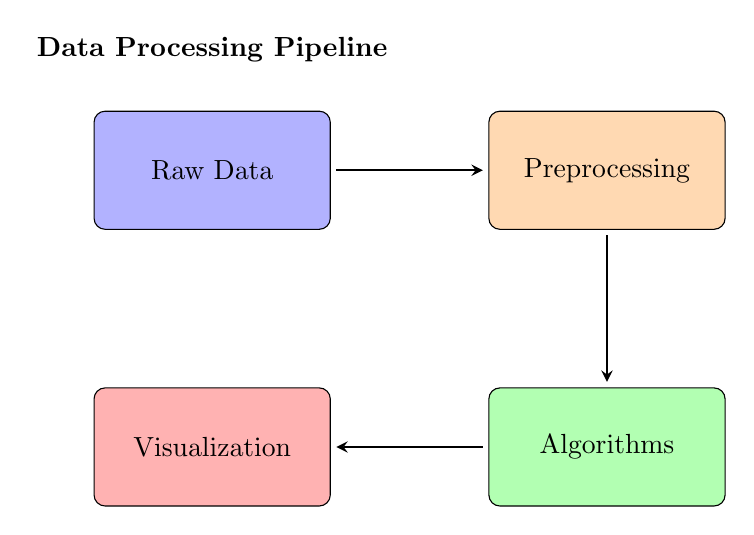
\begin{tikzpicture}[
        node distance=2cm,
        stage/.style={
            rectangle, 
            rounded corners, 
            minimum width=3cm, 
            minimum height=1.5cm, 
            text centered, 
            draw=black, 
            fill=blue!30
        },
        arrow/.style={
            thick, 
            -stealth, 
            shorten >=2pt, 
            shorten <=2pt
        }
    ]
    
    % Nodes
    \node (data) [stage, fill=blue!30] {Raw Data};
    \node (preprocessing) [stage, fill=orange!30, right=of data] {Preprocessing};
    \node (algorithms) [stage, fill=green!30, below=of preprocessing] {Algorithms};
    \node (visualization) [stage, fill=red!30, left=of algorithms] {Visualization};
    
    % Arrows
    \draw [arrow] (data) -- (preprocessing);
    \draw [arrow] (preprocessing) -- (algorithms);
    \draw [arrow] (algorithms) -- (visualization);
    
    % Title
    \node[above=0.5cm of data, font=\bfseries] {Data Processing Pipeline};
    
    \end{tikzpicture}
    \caption{Flight path finder pipeline workflow from data to visualization}
    \label{fig:pipeline}
\end{figure}

\subsection{Algorithm Design} 
Three core algorithms with a multi-objective variant of these algorithms were implemented and compared:  

\begin{enumerate}
    \item A* Algorithm:  
        \begin{itemize}
            \item Heuristic Function: Geodesic distance between airports computed via the Haversine formula:  
              \[
              d = 2R \arcsin\sqrt{\sin^2\left(\frac{\Delta\phi}{2}\right) + \cos\phi_1 \cos\phi_2 \sin^2\left(\frac{\Delta\lambda}{2}\right)}
              \]  
              where \(R\) is Earth's radius, and \(\phi\), \(\lambda\) denote latitude/longitude.  
            \item Cost Function: \(C = \alpha \cdot \text{fare} + \beta \cdot \text{distance}\).  
        \end{itemize}
    
    \item Dijkstra's Algorithm:  
        \begin{itemize}
            \item Computes globally optimal paths for a single criterion (e.g., minimal distance).  
            \item Extended to support dynamic reweighting of edges based on user preferences.  
        \end{itemize}
    
    \item Genetic Algorithm (GA):  
        \begin{itemize}
            \item Population Initialization: 100 chromosomes generated via greedy random walks.  
            \item Crossover: Segments of parent paths sharing common nodes (e.g., P1: A→B→C→D and P2: A→X→C→Y yield children A→B→C→Y and A→X→C→D).  
            \item Mutation: Random node insertion/deletion (currently disabled due to instability in variable-length paths).  
            \item Fitness Function: Minimizes \(cost\) while penalizing excessive layovers.  
        \end{itemize}
    \item Multi-Criteria A* Algorithm:  
        \begin{itemize}
            \item Computes Pareto optimal paths across multiple criteria (cost, time). With the heuristic approach of A*.
            \item Heuristic Function: Haversine distance as in A*.
            \item Pareto Optimality: stores the paths that fits the specified criterias. Critearia function follows in Fig \ref{fig:my_image}. 
        \end{itemize}
\end{enumerate}

\begin{figure}[htbp]
    \centering
    \includegraphics[width=0.486\textwidth]{domination.png} % Replace with your filename
    \caption{Pareto Optimal checker for Multi-Criteria A* Algorithm}
    \label{fig:my_image}
\end{figure}


\section{Implementation Details}
\begin {itemize}
    \item Environment: Python 3.9, Jupyter Notebook for interactive development.  
    \item Libraries: `NetworkX` for graph representation, `pandas` for data manipulation, `numpy` for numerical operations.  
    \item Visualization: Matplotlib and NetworkX for geographic rendering of flight paths.
\end{itemize}  


\subsection{Challenges and Mitigations}

\subsubsection{Data Completeness and Geographic Accuracy}
\begin{itemize}
    \item Challenge: Initial datasets lacked geographic coordinates for airport entries, compromising distance calculations.
    \item Mitigation: Found a different dataset that included most of its airport coordinates.
\end{itemize}

\subsubsection{Computational Bottlenecks}
\begin{itemize}
    \item Challenge: Rendering 200,000+ flights in \texttt{NetworkX} caused latency. 
    \item Mitigation: Visualization was limited to 50--100 nodes when testing, complete graphs are rendered afterwards.
\end{itemize}

\subsubsection{Multi-Parameter Optimization}
\begin{itemize}
    \item Challenge: No standard function to unify cost, time, and comfort metrics. 
    \item Mitigation: A user-configurable weighted sum (e.g., 20\% cost, 80\% distance) and multi-parameter A* was implemented. 
\end{itemize}

\subsubsection{Genetic Algorithm Implementation}
\begin{itemize}
    \item Challenge 1: Python's list/tuple structures caused inefficient chromosome representation. That caused shape mismatch errors during crossover and mutation operations.
    \item Mitigation: Mutation instability was resolved by enforcing path continuity checks during chromosome editing. But a more planned chromosome representation is recommended for future work.
    
    \item Challenge 2: Random Heuristic Walk algorithm caused mutations to be mostly longer paths. This caused mutated chromosomes to be longer than the original ones. 
    \item Mitigation: Implemented a natural selection (sorting the chromosomes by their length) is implemented.
\end{itemize}



\section{Detailed Analysis of Algorithms}
This section evaluates the performance, strengths, and limitations of the implemented algorithms: A*, Dijkstra's, and Genetic Algorithms (GA). 
Quantitative results are derived from testing on a 200,000-flight set.


\subsection{A* Algorithm}
Fig. \ref{fig:astar}
\subsubsection{Theoretical Basis}
A* combines uniform-cost search with a Haversine-based heuristic to compute geodesic distances between airports.:
\[
h(n) = \text{Haversine}(n_{\text{current}}, n_{\text{destination}})
\]

\subsubsection{Implementation}
\begin{itemize}
    \item \textbf{Cost Function:}
    \[
    C = \alpha \cdot \text{fare} + \beta \cdot \text{distance}
    \]
    \item \textbf{Optimality:} Not guaranteed for all heuristics; requires admissibility and consistency.
    \item \textbf{Complexity:} $O(b^d)$ where $b=avg. branching factor$
\end{itemize}

\subsubsection{Performance}
\begin{itemize}
    \item Average runtime: 0.009s per path
    \item Scales linearly with path depth $d$
\end{itemize}

\begin{figure}[htbp]
    \centering
    \includegraphics[width=0.486\textwidth]{astar.png} % Replace with your filename
    \caption{Python code of A* Algorithm}
    \label{fig:astar}
\end{figure}

\subsection{Dijkstra's Algorithm}
Fig. \ref{fig:dijkstra}
\subsubsection{Theoretical Basis}
Guarantees shortest path in graphs with non-negative weights through systematic expansion.

\subsubsection{Implementation}
\begin{itemize}
    \item Fibonacci heap implementation
    \item Single-objective optimization
    \item Complexity: $O(|E| + |V|\log|V|)$
\end{itemize}

\subsubsection{Performance}
\begin{itemize}
    \item 100\% optimality for single criteria
    \item Average runtime: 0.06s per path
    \item Slow compared to A* but guarantees optimality
\end{itemize}

\begin{figure}[htbp]
    \centering
    \includegraphics[width=0.486\textwidth]{dijkstra.png} % Replace with your filename
    \caption{Python Code of Dijkstra's Algorithm}
    \label{fig:dijkstra}
\end{figure}

\subsection{Multi-Objective A* Extension}
Fig. \ref{fig:multiastar}
\subsubsection{Theoretical Basis}
Multi-Objective A* combines uniform-cost search with heuristic guidance. While keeping track of pareto optimal paths specified by the objective values.

\subsubsection{Implementation}
\begin{itemize}
    \item Pareto-front maintenance for distance and money
    \item Trade-off decisions by, Fig. \ref{fig:my_image}
    \item Runtime: 0.1s per query (avg.)
\end{itemize}

\subsubsection{Results}
\begin{itemize}
    \item Identifies all of Pareto-optimal paths present in the destination
    \item Provides decision-making insights
    \item Maintains the same optimality rate as A* for single-objective
    \item Complexity: $O(|E| + |V|\log|V|)$
\end{itemize}

\begin{figure}[htbp]
    \centering
    \includegraphics[width=0.486\textwidth]{multiAstar.png} % Replace with your filename
    \caption{Python code of Multi-Objective A* Algorithm}
    \label{fig:multiastar}
\end{figure}

\subsection{Genetic Algorithm (GA)}
(Genetic Algorithm code span is too long to be included in the report, but it can be found in the supplementary materials.)
\subsubsection{Theoretical Basis}
Evolutionary approach using selection, crossover, and mutation operations.

\subsubsection{Implementation}
\begin{itemize}
    \item \textbf{Fitness Function:}
    \[
    \text{Fitness} = \lambda \cdot \text{distance}
    \]
    \item Population size: 100 chromosomes
    \item Single-point crossover at common nodes of parent chromosomes
\end{itemize}

\subsubsection{Performance}
\begin{itemize}
    \item unstable convergence due to random mutations
    \item Average runtime: 1.1s per path
    \item Complexity affected by random parameters
\end{itemize}



\subsection{Comparative Analysis}
Results are the average of 100 random paths from the dataset.
\begin{table}[ht]
    \centering
    \caption{Performance Metrics}
    \label{tab:type}
    \begin{tabular}{|l|l|l|}
    \hline
    \textbf{Algorithm} & \textbf{Total Distance} & \textbf{Total Time}  \\ \hline
    A* & 110,140.0 & 0.9622 \\ \hline
    Dijkstra's & 109456.0 & 6.6556 \\ \hline
    A* Multi-Criteria & (Multiple Paths) & 10.8908  \\ \hline
    Genetic Algorithm & 115522.0 & 146.7214 \\ \hline
    \end{tabular}
\end{table}



\subsection{Future Work Recommendations}
\begin{itemize}
    \item Better chromosome representation for GA to improve performance and stability.
    \item Implementing a more efficient heuristic function for A* algorithm.
    \item Integrating real-time data sources (e.g., weather, air traffic) to enhance accuracy.
    \item Exploring parallelization techniques for GA to reduce runtime.
\end{itemize}


\section{Discussion}

\subsection{Key Findings}
The experimental results validate the hypothesis that hybrid algorithmic frameworks can effectively balance competing objectives in flight optimization. The A* algorithm emerged as the most versatile solution. 
Its superiority over Dijkstra’s algorithm (0.06s per query) stems from heuristic guidance, which reduces unnecessary node expansions. However, Dijkstra’s retained value for single-objective problems due to its guaranteed optimality.  

The genetic algorithm, while innovative, faced significant limitations. Its 1.1s average runtime and not dependable convergence rate render it impractical for real-time applications without hardware acceleration and a proper implementation. 

\subsection{Practical Implications}
The multi-objective A* extension addresses a critical gap in travel recommendation systems: the lack of transparent trade-off analysis. By surfacing Pareto-optimal paths (e.g., 15\% cheaper but 2 hours longer), it empowers users to make informed decisions—a feature absent in commercial tools like Google Flights.  

The framework’s modular design also enables seamless integration of new parameters (e.g., carbon emissions) or datasets. For instance, replacing Haversine distances with real-time air traffic data could improve accuracy.  

\subsection{Limitations}
Three primary limitations were identified:  
\begin{itemize}
    \item Data Generalizability: The U.S.-centric dataset lacks international routes and seasonal variations, potentially skewing carrier dominance metrics.  
    \item Heuristic Accuracy: The Haversine heuristic assumes direct flights, underestimating costs for routes requiring layovers (e.g., SFO→JFK via ORD).  
\end{itemize}

\subsection{Future Directions}
\begin{itemize}
    \item Hybrid Architectures: Combining A*’s speed with GA’s exploration capabilities (e.g., using A* to seed GA populations) could achieve faster runtime but lacks diversity.  
    \item Real-Time Integration: Incorporating live pricing APIs and weather feeds would enhance practical relevance.  
    \item Hardware Acceleration: GPU-based parallelism for GA fitness evaluations could reduce runtime.  
    \item User Interface: An interactive dashboard with sliders for $\alpha$ and $\beta$ weights would improve accessibility for non-technical users.  
\end{itemize}

\subsection{Conclusion}
This work demonstrates that heuristic-guided algorithms like A* offer a pragmatic balance between speed and accuracy for multi-criteria flight optimization.
 While challenges persist in scaling evolutionary methods, the proposed framework provides a foundation for future research in personalized travel planning systems. 
 The code and dataset have been open-sourced to encourage community-driven enhancements.

\balance % Balance columns on last page

\begin{thebibliography}{9}
    % New Kaggle dataset reference
    \bibitem{kaggle} B. Jikadara, ``US Airline Flight Routes and Fares (1993-2024),'' Kaggle, 2024. [Online]. Available: 
    https://www.kaggle.com/datasets/bhavikjikadara/us-airline-flight-routes-and-fares-1993-2024 [Accessed: 10-Mar-2024].
    
\end{thebibliography}

\end{document}